\section{The Standard Model of Particle Physics}

The Standard Model \cite{Spiesberger:2000ks} is an effective description of all known fundamental particles.  Despite this criticism, the Standard Model provides a valid framework for the description of Nature, from microscopic scales up to cosmological distances.The Standard Model consists of three components.

this is the standard model. Is great but is also crap (cit. Jori)

\subsection{Matter}

The first component states that the basic constituents of matter are leptons and quarks which are realized in three families of identical structure. The entire ensemble of these constituents has been identified experimentally. Table \ref{table:fermions} shows all the fermions of the Standard Model and their charges, arranged in the three families.

	\begin{figure}[tbh!]
		\begin{center}
			
			\begin{tabular}{ | c | c | c | c | c |}
				\hline
				& 1st Generation & 2 Generation & 3rd Generation & charge \\ \hline \hline
				& & & & \\
				leptons & $\left( \begin{array}{c} \nu_{e} \\ e \end{array} \right)_{L}$ & $\left( \begin{array}{c} \nu_{\mu} \\ \mu \end{array} \right)_{L}$ & $\left( \begin{array}{c} \nu_{\tau} \\ \tau \end{array} \right)_{L}$ & \begin{tabular}{@{}c@{}}weak \\ weak, electromagnetic\end{tabular} \\
				& & & & \\
				 & $e_{R}$& $\mu_{R}$& $\tau_{R}$& electromagnetic\\ 
				 & & & & \\
				 \hline
				 & & & & \\
				leptons & $\left( \begin{array}{c} u \\ d \end{array} \right)_{L}$ & $\left( \begin{array}{c} c \\ s \end{array} \right)_{L}$ & $\left( \begin{array}{c} t \\ b \end{array} \right)_{L}$ & weak, electromagnetic, strong \\
				& & & & \\
				& $u_{R}, d_{R}$& $c_{R}, s_{R}$& $t_{R}, b_{R}$& electromagnetic, strong\\
				& & & & \\ 
				\hline
				\hline
			\end{tabular}
			\caption{Fermions of the Standard Model and their charges, arranged in the three generations. Only the left-handed fermions interact weakly and are arranged in doublets. The right-handed fermions are singlets. The right-handed neutrinos are not present in this table, as they do not interact with one of the forces of the Standard Model.}
			\label{table:fermions}
		\end{center}
	\end{figure}
	
	\begin{figure}[tbh!]
		\centering
		\begin{tabular}{cc}
			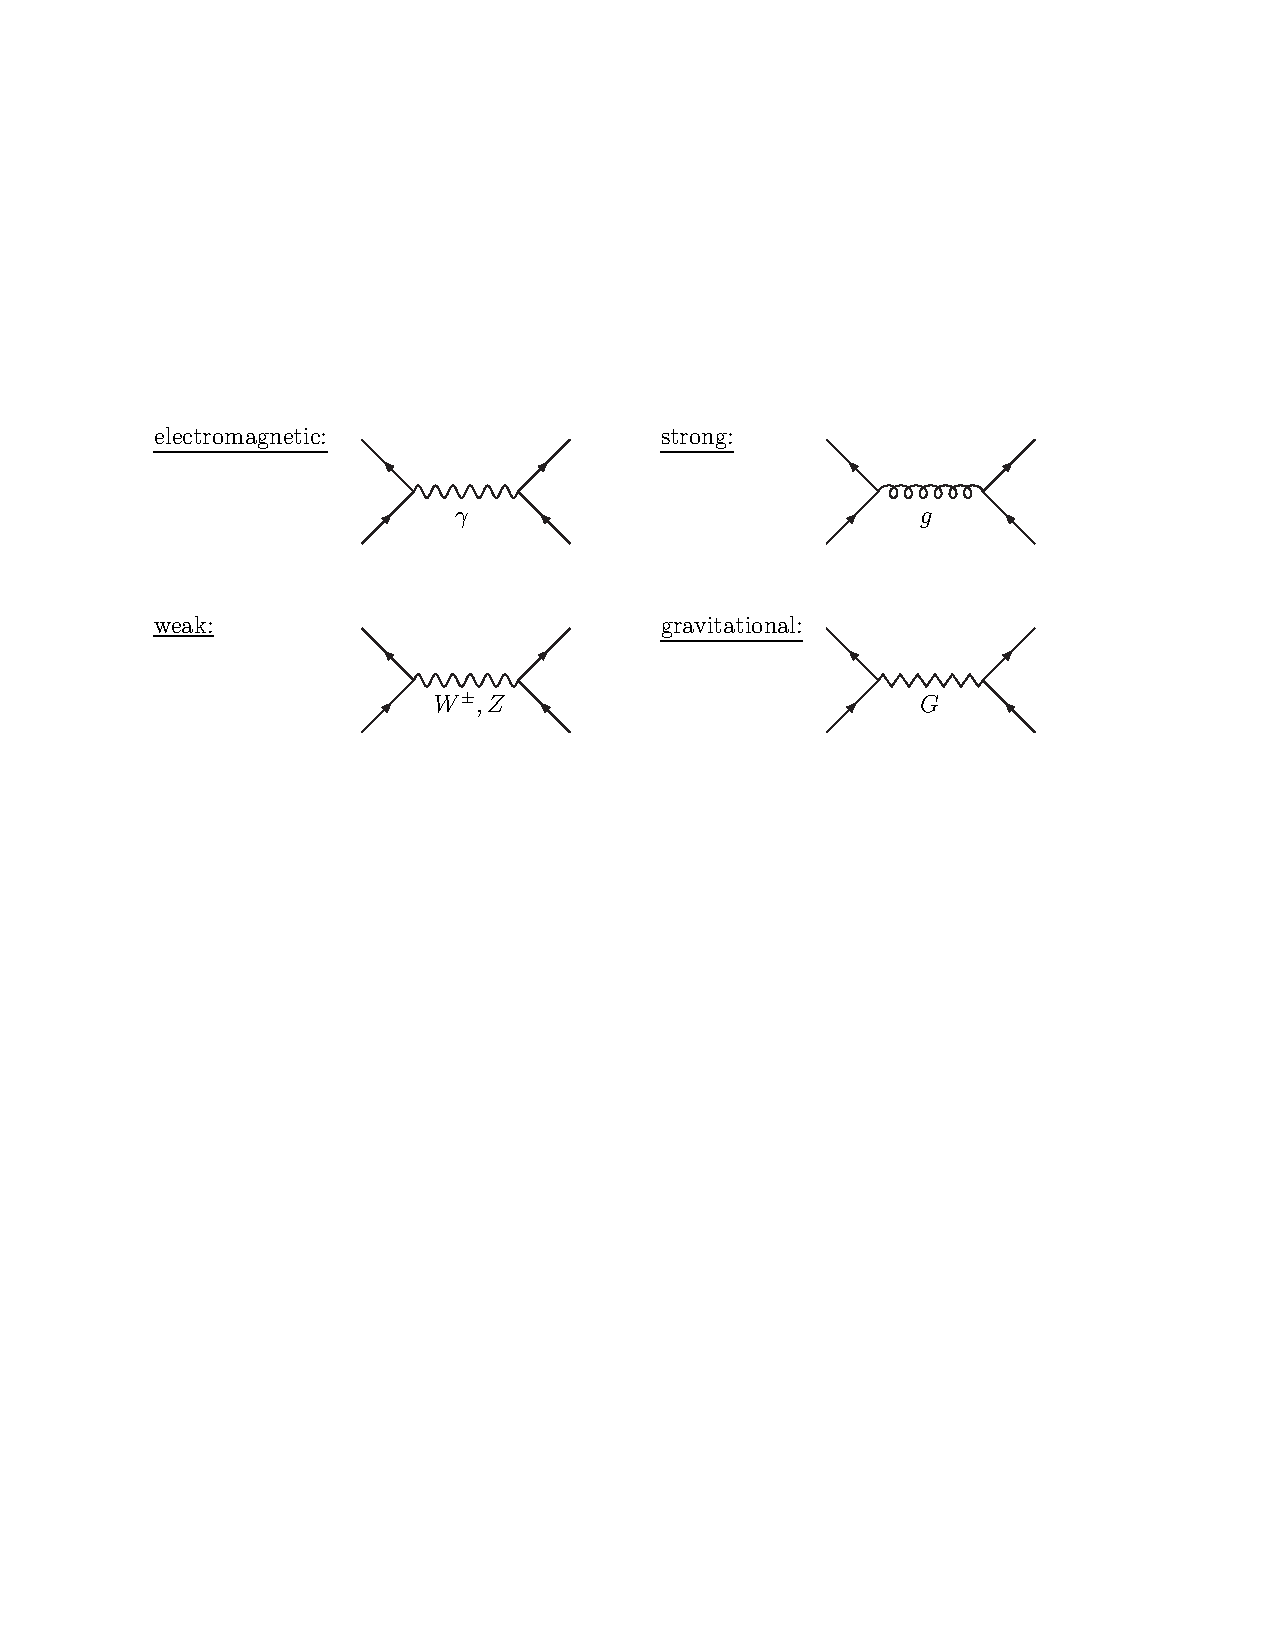
\includegraphics[width=0.75\textwidth]{theory/pics/SM_forces.pdf}
		\end{tabular}
		\caption{The four fundamental forces in nature as described by the Standard Model.}
		\label{fig:SM_forces}
	\end{figure}

\subsection{Interactions}

The interactions are mediated by bosons. They are the quanta of the gauge fields, and couple to the corresponding charges. The interactions are described by symmetry transformations U of the group SU(n). They are unitary (UU† = 1) and special (det(U) = 1). An operator


-----------------------------
	
The second component are the four different forces acting between the leptons and quarks. The electromagnetic and weak forces are unified in the Standard Model. The fields associated with these forces, as well as the fields associated with the strong force, are spin-1 fields, describing the photon \ensuremath{\gamma}, the electroweak gauge bosons \W and \Z, and the gluons g. The interactions of the force fields with the fermionic constituents of matter as well as their self-interactions are described by Abelian and non-Abelian \ensuremath{SU(3) \times SU(2) \times U(1)} gauge theories. The experimental exploration of these fundamental gauge symmetries is far advanced in the sector of lepton/quark-gauge boson interactions, yet much less is known so far from experiment about the self-interactions of the force fields. The gravitational interaction is mediated by a spin-2 field, describing the graviton G, with a character quite different from spin-1 gauge fields. The gravity sector is attached ad hoc to the other sectors of the Standard Model, not properly formulated yet as a quantum phenomenon. Figure \ref{fig:SM_forces} shows the four fundamental forces in nature as described by the Standard Model.



\begin{figure}[tbh!]
	\centering
	\begin{tabular}{cc}
		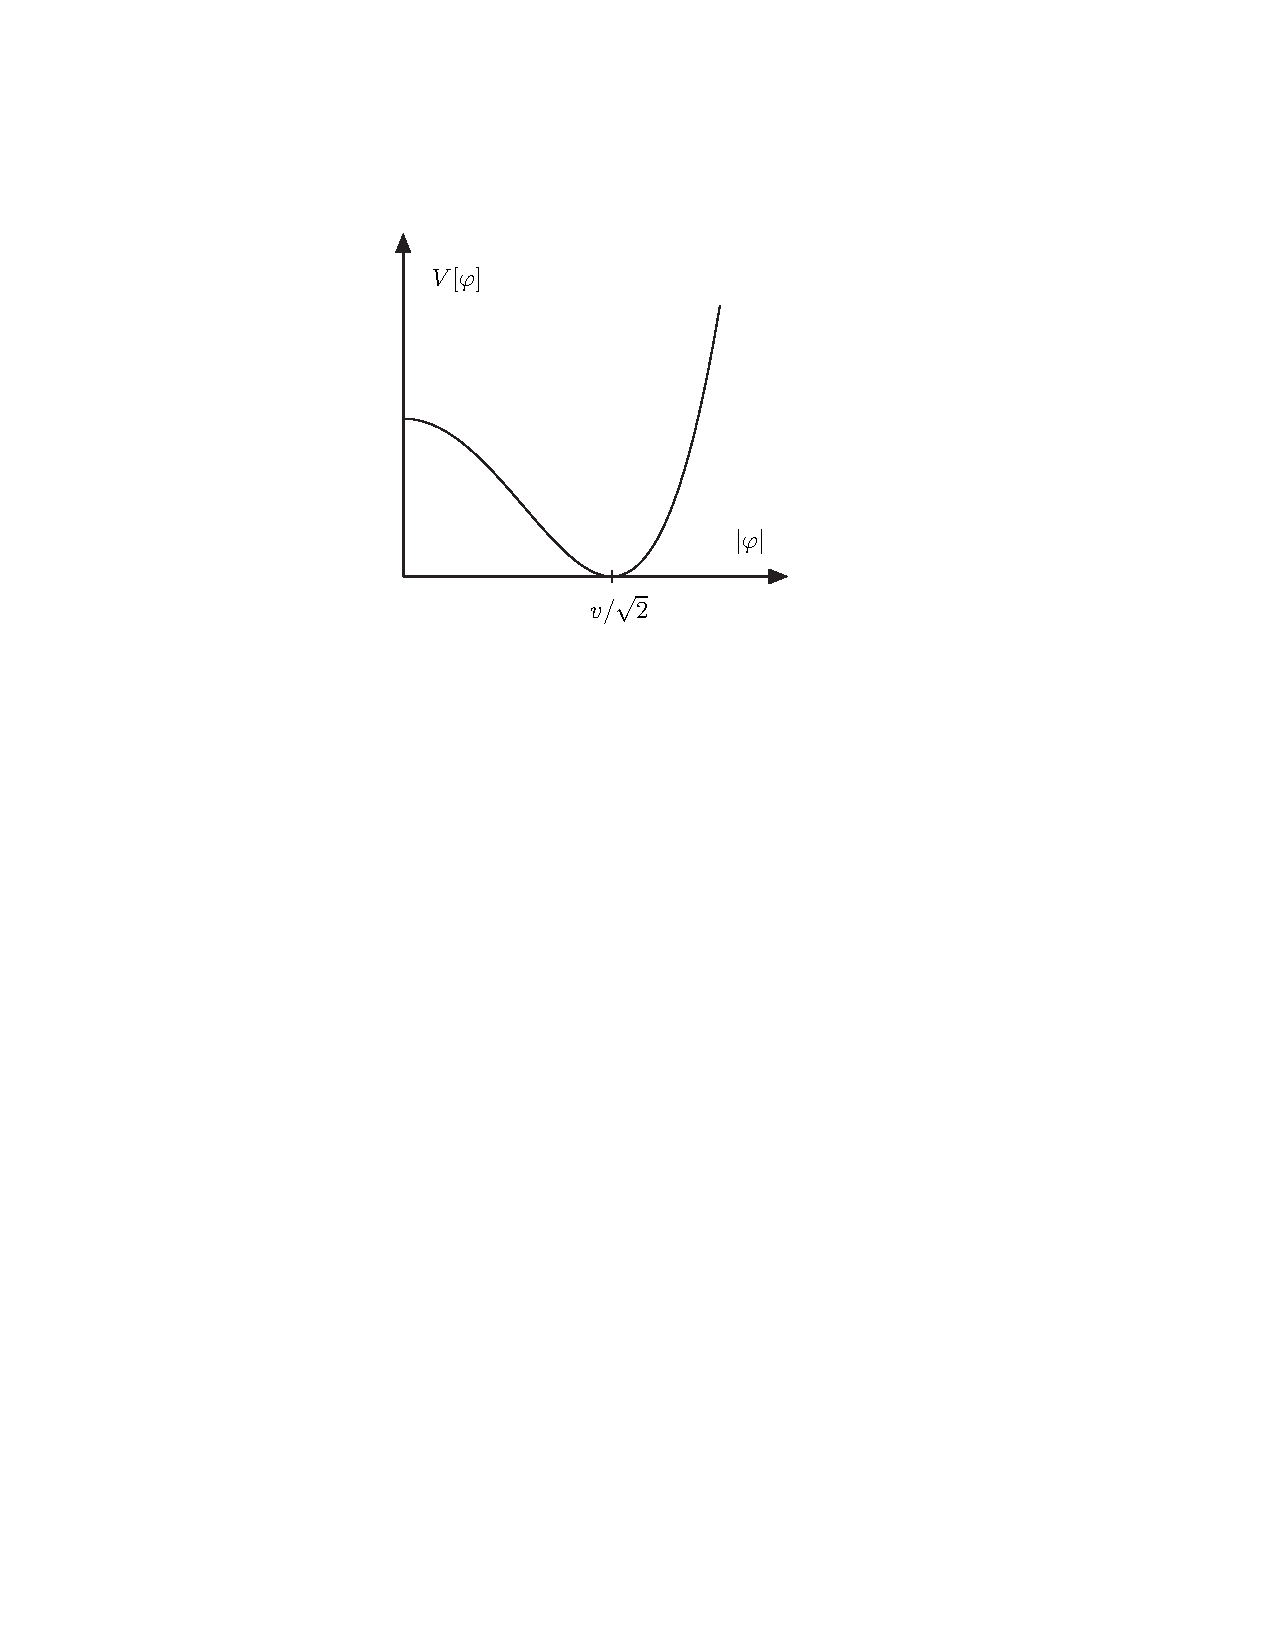
\includegraphics[width=0.75\textwidth]{theory/pics/higgs_potential.pdf}
	\end{tabular}
	\caption{The Higgs potential of the Standard Model.}
	\label{fig:higgs_potential}
\end{figure}


\subsection{The Higgs Mechanism}
\label{higgs_mechanism}

The starting point is the promotion from a global gauge transformation to the minimal to a point-dependent gauge transformation to the minimal Lagrangian . This requires in addition to the starting complex scalar field also a vectorial field $A_{\mu}$ analog to the electromagnetic field. The resulting Lagrangian is:

\begin{equation}
\mathcal{L} = (D_{\mu}\phi)^{\dagger} D^{\mu}\phi - V (\phi) - \dfrac{1}{4}F_{\mu\nu}F^{\mu\nu}\
\label{eq::lagrangian_min}
\end{equation}
\begin{equation}
V(\phi)=\mu^{2}\phi^{\dagger}\phi+\lambda(\phi^{\dagger}\phi)^{2} -\epsilon\phi^{\dagger} -\epsilon^{*}\phi
\end{equation}

\begin{equation}
D^{\mu} = \partial^{\mu} - ieA^{\mu}
\end{equation}

\begin{equation}
F^{\mu\nu} =\partial^{\nu}A^{\mu} - \partial^{\mu}A^{\nu}
\end{equation}

where $\epsilon \rightarrow 0$, $\mathcal{L}$ is invariant under gauge transformations:

\begin{equation}
\phi(x) \rightarrow e^{i\alpha(x)}\phi(x); \phi(x)^{\dagger} \rightarrow e ^{-i\alpha(x)}\phi(x)^{dagger}
\end{equation}

\begin{equation}
A^{\mu} \rightarrow A^{\mu} + \dfrac{1}{e}\partial^{\mu}\alpha(x)
\label{eq::a_tranform}
\end{equation}

Where $\alpha(x)$ is an arbitrary function of x and $e$ is a new coupling constant, identical to the electrical charge in case $A_{\mu}$ is identified as the electromagnetic field. In order to obtain a stable theory $\lambda > 0$, however $\mu^{2}$ can have two cases depending on the sign choice:
 
1. $\mu^{2} > 0$. The energy minimum is at $\phi = 0$ and $A_{\mu} = 0$. The resulting theory consists of:

\begin{enumerate}
	\item a charged particle and its anti-partner, both with mass $\mu^{2} \neq 0$;
	\item a massless particle with spin 0, similar to the photon.
\end{enumerate}

For small values of $\lambda$ and $e$ the Lagrangian describes the interactions between scalar particles with the electromagnetic field (trough the coupling constant $e$) and their self-interactions (through the couping constant $\lambda$).

2. $\mu^{2} < 0$. The energy minimum is at $A_{\mu} = 0$, so in  case $\epsilon \rightarrow 0$:

\begin{equation}
V(\bar{\phi})=min ; \quad \bar{\phi}=\eta= 2\lambda +O(\epsilon)
\end{equation}
 
 in order to study the  variations around the minimum $\phi$ is defined as:

\begin{equation}
 \phi=\eta + \dfrac{\sigma_{1}(x) + i\sigma_{2}(x)}{\sqrt{2}} 
\end{equation}

and is used into the minimal Lagrangian \ref{eq::lagrangian_min}.

The particle masses spectrum is obtained from the fields $\sigma_{i}$ and $A_{\mu}$ quadratic terms. In addition, for $\alpha \rightarrow 0$, $\phi$ transforms as:

\begin{equation}
\phi \rightarrow \phi + i\alpha\phi = \eta + \dfrac{\sigma_{1}(x) + i\sigma_{2}(x)}{\sqrt{2}} + i\eta\alpha(x)
\end{equation}

or rather:

\begin{equation}
\sigma_{1}(x) \rightarrow \sigma^{\prime}_{1}(x) = σ_{1}(x); \quad \sigma_{2}(x) \rightarrow \sigma^{\prime}_{2}(x) = \sigma_{2}(x) + \sqrt{2}\eta\alpha(x)
\end{equation}

$A_{\mu}$ transforms following \ref{eq::a_tranform}. The $\sigma_{2}$ field non-homogeneously transforms by the addition of an $\alpha$ term, arbitrary function of $x$. In case of the given $\sigma_{i}(x)$ and $A_{\mu}$ where:

\begin{equation}
\alpha(x) = -\dfrac{σ\sigma_{2}(x)}{\sqrt{2}\eta}
\end{equation}

resulting in:

\begin{equation}
\sigma^{\prime}_{2}(x) = 0
\label{eq::unitary_gauge}
\end{equation}

the $\sigma_{2}$ filed can be crossed out in case of a gauge symmetry. The gauge identified by \ref{eq::unitary_gauge} is commonly known as unitary gauge.

\begin{figure}[tbh!]
	\centering
	
	\begin{tabular}{cc}
		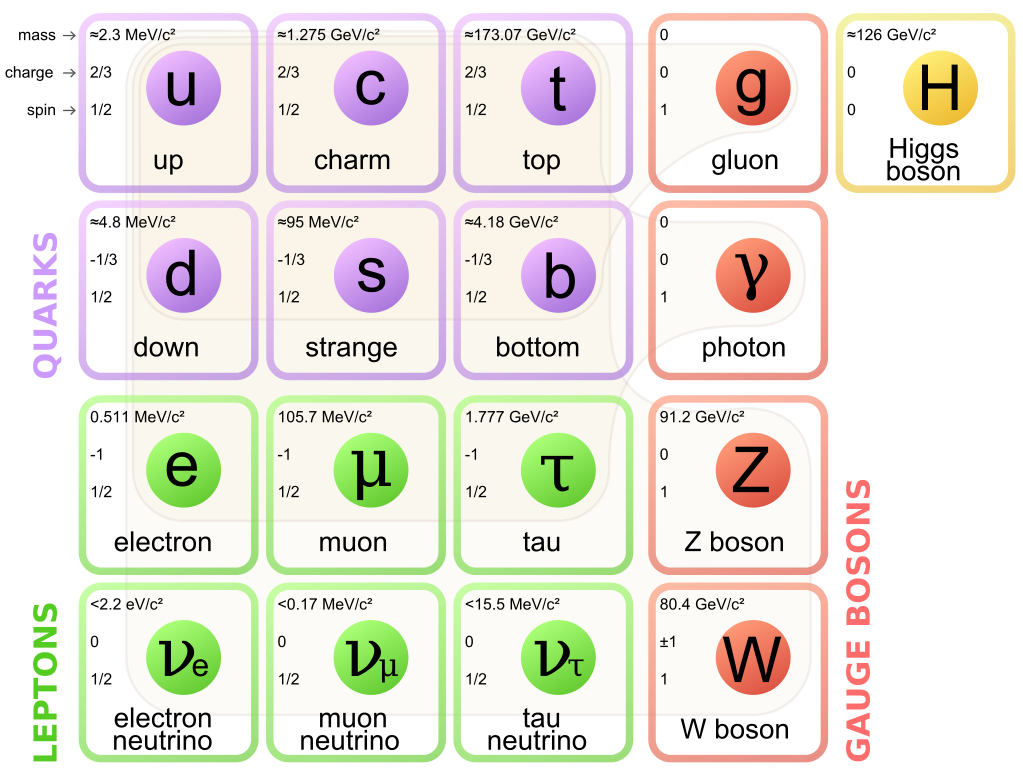
\includegraphics[width=0.75\textwidth]{theory/pics/SM_particles.png}
	\end{tabular}
	\caption{The Standard Model of elementary particles consists of  12 fundamental fermions and 4 fundamental bosons. Brown loops indicate which bosons (red) couple to which fermions (purple and green).}
	\label{fig:SM_particles}
\end{figure}

\begin{figure}[tbh!]
	\centering
	\begin{tabular}{cc}
		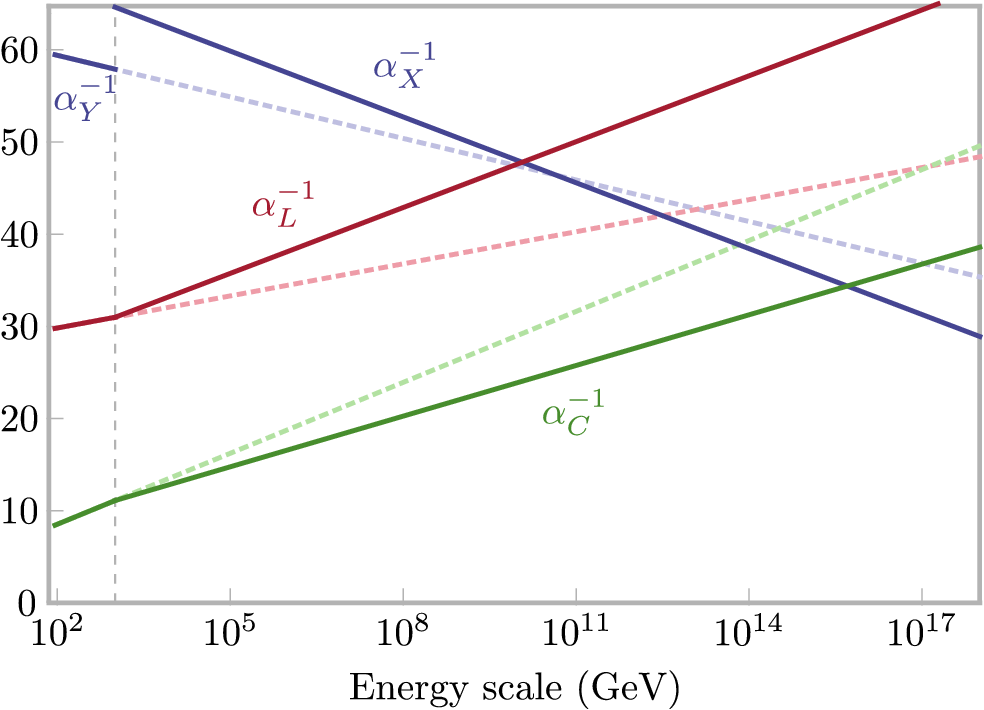
\includegraphics[width=0.75\textwidth]{theory/pics/gauge_unification.png}
	\end{tabular}
	\caption{Running of the gauge coupling constants in the SM (dashed lines) and in the model in Ref.~\cite{PhysRevD.90.013005} (solid lines). Here the $M_{331}$ scale is set to 11~TeV}
	\label{fig:gauge_unification}
\end{figure}

\subsection{The bosonic masses}

The starting point is a theory based on the $SU(2)_{L} \oplus U(1)_{Y}$ symmetry:

\begin{equation}
\mathcal{L}_{eW} = \bar{l}i\gamma^{\mu} D_{\mu}l + \bar{e}_{R}i\gamma^{\mu}D_{\mu}e_{R} − \dfrac{1}{4}[W_{\mu\nu}W^{\mu\nu} +B_{\mu\nu}B^{\mu\nu}]
\label{eq::lagrangian_ew}
\end{equation}

with the leptonic fields defined as:

\begin{equation}
\binom{(\nu_{e})_{L}}{e_{L}}_{Y=−2} ; \quad (e_{R})_{Y=−2}
\label{eq::fields_scheme}
\end{equation}

and the covariant derivatives and tensors defined as:

\begin{equation}
D_{\mu}l = [\partial_{\mu} + igW_{\mu} \dfrac{\tau}{2}  + ig^{\prime}(-\dfrac{1}{2})B_{\mu}]l 
\end{equation}

\begin{equation}
D_{\mu}e_{R} = [\partial_{\mu} + ig^{\prime}(-1)B_{\mu}]e_{R}
\end{equation}

\begin{equation}
W_{\mu\nu} =\partial_{\nu}W_{\mu} - \partial_{\mu}W_{\nu} 
\end{equation}

\begin{equation}
B_{\mu\nu} =\partial_{\nu}B_{\mu} - \partial_{\mu}B_{\nu} 
\end{equation}

At this stage the theory describes massless fermions and vectorial fields. The introduction of a scalar field triggers a symmetry breaking while keeping the electromagnetism gauge still intact:

\begin{equation}
SU(2)_{L} \oplus U(1)_{Y} \rightarrow U(1)_{em}
\end{equation}

The optimal choice in order to generate the electron and quarks mass is to choose a $SU(2)_{L}$ doublet with $Y = +1$: 

\begin{equation}
\phi = \binom{(\phi{+})_{L}}{\phi^{0}}_{Y=+1}
\label{eq::su2_doublet}
\end{equation}

\begin{equation}
D_{\mu}\phi = [\partial_{\mu} + igW_{\mu} \dfrac{\tau}{2}  + ig^{\prime}(+\dfrac{1}{2})B_{\mu}]\phi 
\end{equation}


with the addition of the fully symmetric Higgs doublet to \ref{eq::lagrangian_ew} the total Lagrangian becomes:

\begin{equation}
\mathcal{L}_{tot} = \mathcal{L}_{eW} + \mathcal{L}_{\phi W}
\end{equation}

where:

\begin{equation}
\mathcal{L}_{\phi W} = (D_{\mu}\phi)^{\dagger} (^{\mu}\phi) - V (\phi);
\label{eq::lagrangian_phiW}
\end{equation}

\begin{equation}
V(\phi) = \mu^{2}\phi^{\dagger}\phi + \lambda(\phi^{\dagger}\phi)^{2}
\end{equation}

Following the example shown in Section \ref{higgs_mechanism}, $\phi$ can gain a vacuum expectation term, breaking the symmetry:

\begin{equation}
 \bar{\phi}= < 0|\phi|0 > = \binom{0}{\eta}
 \label{eq::vacuum_expectation}
\end{equation}

where:

\begin{equation}
\eta = \sqrt{\dfrac{-\mu^{2}}{2\lambda}}
\label{eq::eta_value}
\end{equation}

In the \ref{eq::su2_doublet} doublet the electric charge is represented as:

\begin{equation}
Q = 
\begin{pmatrix}
+1 & 0 \\
0 & 0 \\
\end{pmatrix}
\end{equation}

so that the field minimum is invariant under phase transformations associated to $U_{em}(1)$:

\begin{equation}
e^{i\alpha Q} \bar{\phi} = 
\begin{pmatrix}
e^{i\alpha} & 0 \\
0 & 1 \\ 
\end{pmatrix}
\binom{0}{\eta}
= \bar{\phi}
\end{equation}

The symmetry breaking given by $\bar{\phi} \neq 0$ gives the scheme \ref{eq::fields_scheme}.
In order to correctly identify all the particles qa definition of the unitary gauge conditions is mandatory. Knowing that every two-dimensional spinor can transform to a spinor with only a real lower component through a point-dependent gauge transformation. Therefore a given $\phi(x)$
can be defined as:

\begin{equation}
\phi(x) = U(x) \binom{0}{\rho(x)}
\end{equation}

with $\rho(x)$ real and $U(x)$ as matrix of $ SU(2)_{L} \oplus U(1)_{Y}$. 

In the previously defined unitary gauge the Lagrangian \ref{eq::lagrangian_phiW} becomes:

\begin{equation}
\begin{array}{r c l}
\mathcal{L}_{\phi W}&=&\dfrac{1}{2} \partial_{\mu} \sigma \partial^{\mu} \sigma - V \left[ \eta + \dfrac{\sigma(x)}{\sqrt{2}}\right] + g^{2} W_{\mu}^{i}(W^{j})^{\mu} \left[ \bar{\phi} \dfrac{\tau_{i}\tau_{j}}{4}\bar{\phi}\right] +\\
&+&(g^{\prime})^{2} \dfrac{1}{4}\eta^{2} B_{\mu} B^{\mu} + 2 gg^{\prime} W^{3}_{\mu} B^{\mu} \left[ \bar{\phi} \dfrac{\tau_{3}}{4} \bar{\phi} \right]
\end{array}
\end{equation}

By using  \ref{eq::vacuum_expectation} and \ref{eq::eta_value} along with the Pauli's matrixes properties:

\begin{equation}
\begin{array}{c}
 W_{\mu}^{i}(W^{j})^{\mu} \left[ \bar{\phi} \dfrac{\tau_{i}\tau_{j}}{4}\bar{\phi}\right] = \frac{1}{4}\eta^{2} W_{\mu}W^{\mu} \\

 W^{3}_{\mu} B^{\mu} \left[ \bar{\phi} \dfrac{\tau_{3}}{4} \bar{\phi} \right] = - \dfrac{1}{4} \eta^{2} W^{3}_{\mu}B^{\mu}
 \end{array}
\end{equation}

from the quadratic terms is possible to get the masses value:

\begin{equation}
\begin{array}{c}
W_{\mu}^{i}(W^{j})^{\mu} \left[ \bar{\phi} \dfrac{\tau_{i}\tau_{j}}{4}\bar{\phi}\right] = \frac{1}{4}\eta^{2} W_{\mu}W^{\mu} \\

W^{3}_{\mu} B^{\mu} \left[ \bar{\phi} \dfrac{\tau_{3}}{4} \bar{\phi} \right] = - \dfrac{1}{4} \eta^{2} W^{3}_{\mu}B^{\mu}
\end{array}
\end{equation}

which becomes:

\begin{equation}
\begin{array}{c}
M^{2}  = \dfrac{1}{2} g^{2} \eta^{2}\\
M_{0}^{2}  = \dfrac{1}{2} (g^{\prime})^{2} \eta^{2}\\
M_{03}^{2}  = -\dfrac{1}{2} gg^{\prime} \eta^{2}
\end{array}
\end{equation}

therefore:

\begin{equation}
\mathcal{M} =  \dfrac{1}{2} \eta^{2}
\begin{pmatrix}
 g^{2} & -gg^{\prime} \\
-gg^{\prime} & (g^{\prime})^{2} \\
\end{pmatrix}
\label{eq::matrix_mass}
\end{equation}

in order to allow the existence of a massless photon $det(\mathcal{M}) = 0$. Knowing that the vacuum configuration in invariant to gauge transformation associated to the electric charge is possible to introduce the massive field $Z_{\mu}$ and the electric field $A_{\mu}$ so that:

\begin{equation}
\begin{array}{c}
Z_{\mu} = cos\theta W^{3}_{\mu} - sin\theta B_{\mu}\\
A_{\mu} = sin\theta W^{3}_{\mu} - cos\theta B_{\mu}

\end{array}
\label{eq::fields_rotation}
\end{equation}

with $\theta$ knows as the electroweak mixing angle. By using the condition that $A_{\mu}$ in the eigen-vector of \ref{eq::matrix_mass} with a zero eigen-value:

\begin{equation}
0 = 
\begin{pmatrix}
g^{2} & -gg^{\prime} \\
-gg^{\prime} & (g^{\prime})^{2} \\
\end{pmatrix}
\binom{sin\theta}{cos\theta}
=
\binom{g^{2} sin\theta - gg^{\prime}cos\theta}{-gg^{\prime}sin\theta + (g^{\prime})^{2}cos\theta}
\label{eq::matrix_rotation}
\end{equation}

the equation in solved for:

\begin{equation}
tan\theta = \dfrac{g^{\prime}}{g}
\label{eq::matrix_solution}
\end{equation}

this condition couples the field $A_{\mu}$ defined in \ref{eq::fields_rotation} with the electron through the electromagnetic current with

\begin{equation}
gsin\theta = g^{\prime} cos\prime = e; 
\end{equation}

The theory symmetry breaking made by Weimber and Salam, based on a symmetric Lagrangian, reproduces the masses spectrum and the couplings on the vectorial fields. All those results has been experimentally confirmed.

\clearpage

\subsection{The fermionic masses}

In order to complete the electro-weak theory the calculation of the fermionic masses is mandatory. Starting with the electron mass taken from the $\mathcal{L}_{m}$ term of the Glashow theory:

\begin{equation}
\mathcal{L}_{m} = m_{e}\bar{e}e = m_{e}(\bar{e}_{L}e_{R} + \bar{e}_{R}e_{L})
\end{equation}

Another invariant Lagrangian is obtainable by combining $\mathcal{L}_{m}$ with the Higgs field, which also has the electro-weak iso-spin of $1/2$. Following the symmetry breaking, $\phi$ gains a constant component, which reproduces the Lagrangian  $\mathcal{L}_{m}$, while the quantum component of $\phi$ gives raise to a new interaction between $\phi$ and the electron. The invariant Lagrangian becomes:

\begin{equation}
\mathcal{L}_{e\phi} = g_{e} (\bar{l}\phi e_{R} + \bar{e}_{R}\phi^{\dagger}l)
\end{equation}

The invariant term $\bar{l}\phi$, under spontaneous symmetry breaking, in the unitary gauge becomes:

\begin{equation}
l\phi = \bar{\nu}_{L}\phi^{+}+ + ¯eLφ0 = ¯eL(η +
σ
√
2
)
\end{equation}

obtaining:



\subsection{Limitations}

\todo{Total Rework}

Although the Standard Model is very successful in describing physics at the electroweak scale, a few questions remain:

\begin{itemize}
	\item Gravity: The Standard Model does not include gravity and already for this reason alone, it cannot be a complete description of nature.
	\item No Electrostrong Unification: The hope of physics in the end is to unify all forces, but while the strong force is well represented by the SU(3), it is not unified with the other forces like it is the case for the electromagnetic and the weak force.
	\item Dark Matter: Astrophysical observations indicate a much greater accumulation of matter in the visible universe than can be explained by baryonic matter [13]. This “dark matter” cannot be explained by neutrinos, which could form only a small fraction of it. The “Modified Newtonian Dynamics” (MOND) [14] was developed in order to explain this excess within the existing theories. It was very successful, especially in explaining the measurement of galaxy rotation curves [15], until the bullet cluster [16] was discovered. Being actually two clusters passing each other, the bullet cluster shows a discrepancy between the center of the masses detected by direct observation and the center of the masses detected by gravitational lensing. This cannot be explained by MOND alone.
	\item WW Scattering: In the Standard Model, the four-vector-boson interaction becomes divergent with rising energy. If the Higgs mechanism turns out to be realized, a new term due to interactions of the vector-bosons with the Higgs is introduced, which cancels out this divergence. But this will only work, if the higgs mass is of the order of 100 GeV, and the WW scattering problem turns into the “fine-tuning” problem.
	\item Neutrino Masses: In the original Standard Model, neutrinos are set to be massless. Experiments showed that neutrinos indeed have non-zero masses [17]. In case of a sterile Dirac neutrino5, the Standard Model can be extended to include massive neutrinos. If it turns out that neutrinos are Majorana particles6, new physics beyond the Standard Model has to be introduced to explain the tiny masses of the neutrinos.
	\item Hierarchy Problem: In the Standard Model, the quantum corrections to the Higgs mass are quadratically divergent. If the Standard Model is assumed to be valid up to the Planck scale7, these corrections are huge compared to the physical Higgs mass.
\end{itemize}

\section{Supersymmetry}

Supersymmetry is one of the most intriguing and fundamental concepts in modern theoretical particle physics. It arises naturally from the combination of the two cornerstones of 20th century physics: quantum mechanics and relativity. Supersymmetry is the unique symmetry that relates the two fundamental kinds of particles: bosons, which act as the carriers of forces, and fermions, which act as the constituents of matter. Supersymmetry transformations are in a sense like the square roots of the coordinate system transformations in special relativity, and consequently supersymmetric quantum field theories have very special, improved properties, compared to ordinary relativistic quantum field theories. If supersymmetry is realized in nature, every fermion in the SM must have a bosonic partner particle and vice versa. No such superpartner particle has been observed so far but there are more and more indications that these particles might show up at the LHC experiments.


\begin{figure}[tbh!]
	\centering
	\begin{tabular}{cc}
		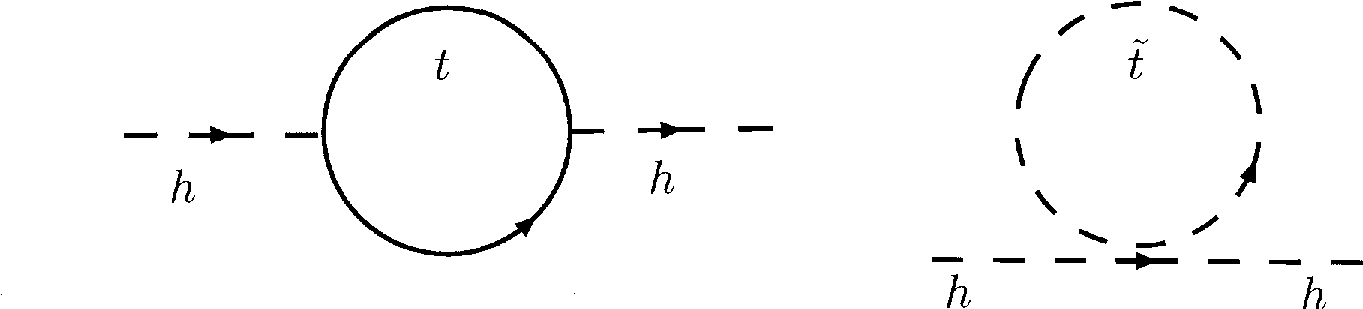
\includegraphics[width=0.75\textwidth]{theory/pics/higgs_loop.png}
	\end{tabular}
	\caption{In SUSY, the correction to Higgs mass by the top quark (L) is inherently cancelled by the contribution from the top quark's supersymmetric partner, the stop (R).}
	\label{fig:higgs_loop}
\end{figure}

\subsection{Motivations}

\subsection{The MSSM}

\begin{figure}[tbh!]
	\centering
	\begin{tabular}{cc}
		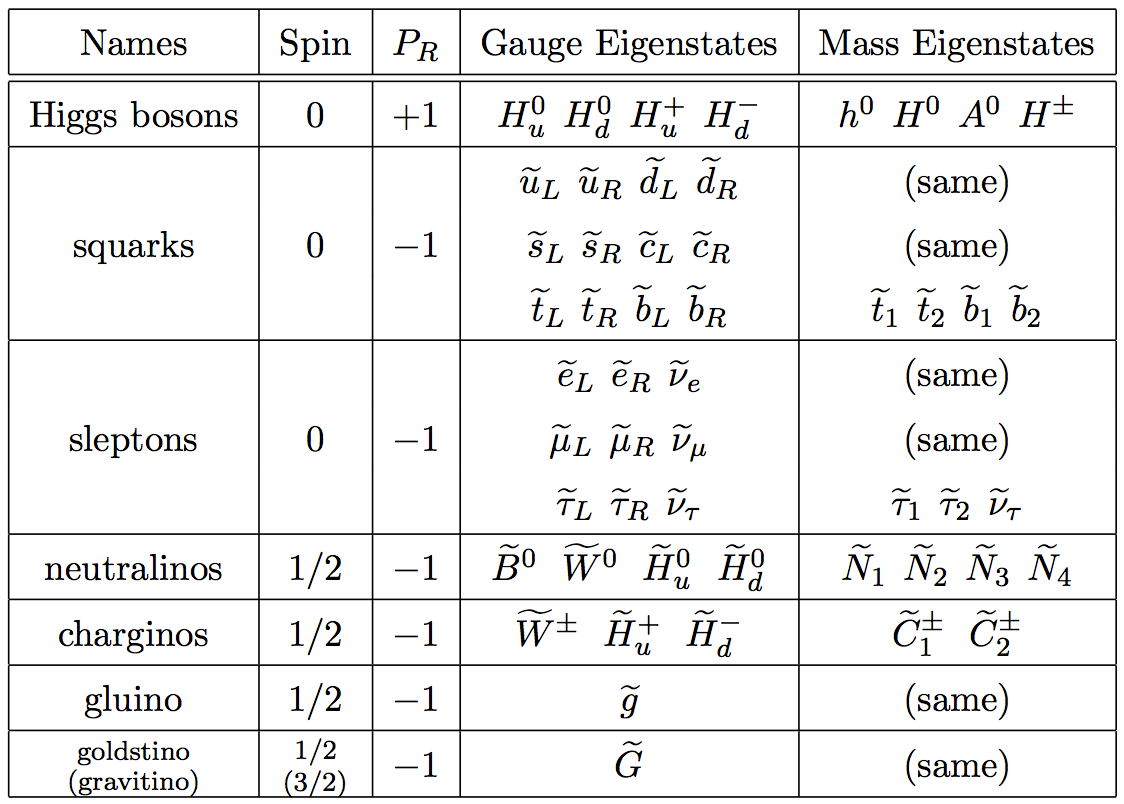
\includegraphics[width=0.75\textwidth]{theory/pics/SUSY_particles_table.png}
	\end{tabular}
	\caption{SUSY particles in MSSM~\protect\cite{Martin:1997ns}}
	\label{fig:SUSY_particles_table}
\end{figure}

\begin{figure}[tbh!]
	\centering
	\begin{tabular}{cc}
		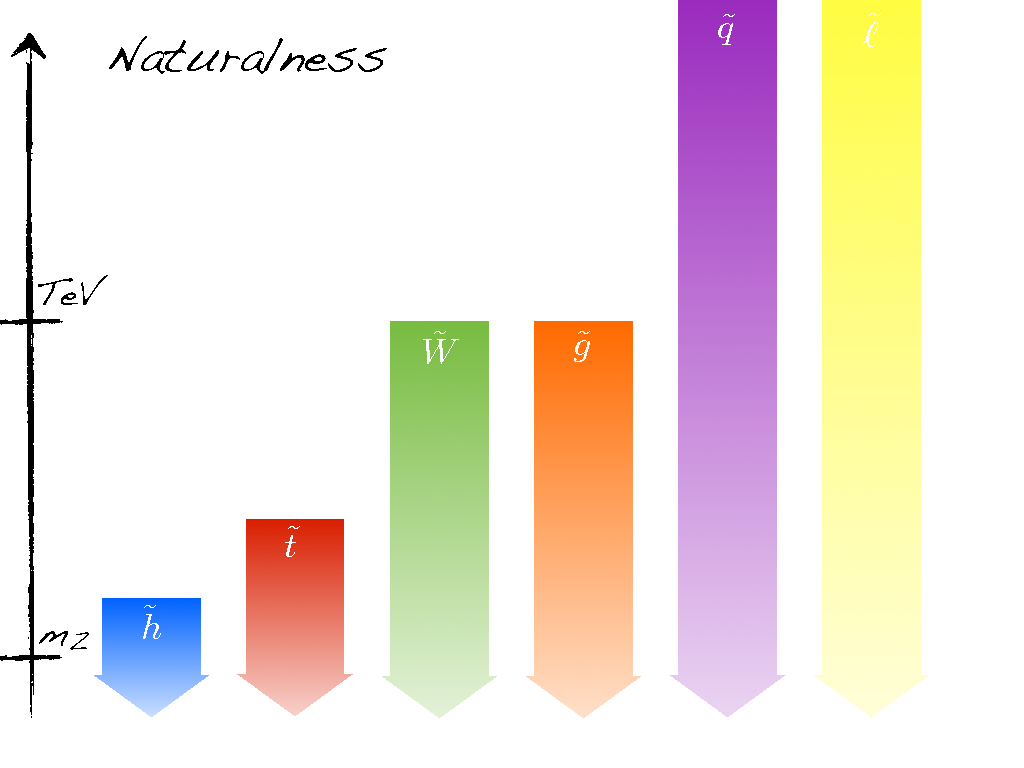
\includegraphics[width=0.75\textwidth]{theory/pics/SUSY_naturalness.png}
	\end{tabular}
	\caption{Cartoon illustration of the mass scales for various sparticles dictated solely by electroweak naturalness with sensitivity parameter $\Delta \lesssim 10$.}
	\label{fig:SUSY_naturalness}
\end{figure}




\subsection{SUSY Signatures at the LHC}
